\section{Results}
\label{results}
The runtime of the algorithms was an unpleasant surprise and is most likely due to the high server usage at the RDC as test runs with a small number of iterations finished quickly on standard laptops. In the final run, each configuration took approximately 23 hours to run, whereas the bagged implementations took 27 hours on average. The binary-encoded variants ran a bit faster as their code was slightly less complex than their real-valued counterparts but still took 21 hours.

Figures \ref{fig:exp12} and \ref{fig:exp34} show the average convergence of each algorithm across all parameter settings. The GA and BSA converge as expected, whereas both PSO implementations show only little improvement to their random initialization. The PBIL is seemingly unable to hold any good solutions over time and tried solutions in a random walk fashion. The parameter setting might be at fault here as the bagged experiments yielded very similar results. %WHERE DID I GET THE PARAMS FROM?

%PSOG SO POORLY
%BAGGING WORSENED HC

\begin{figure}
\centering %CHANGE SUBCAPTION
	\begin{subfigure}{.5\textwidth}
		\centering
		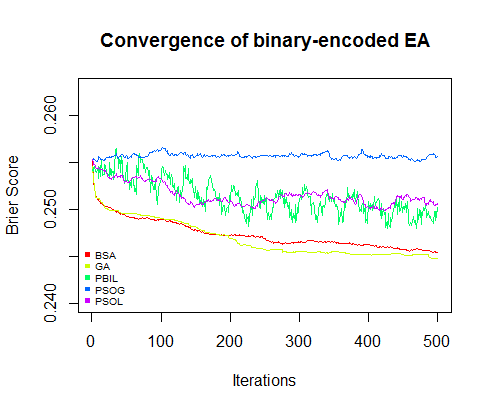
\includegraphics[width=\linewidth]{Conv_N_bin_EA}
		%\caption{A subfigure}
		\label{fig:nb}
	\end{subfigure}%
	\begin{subfigure}{.5\textwidth}
		\centering
		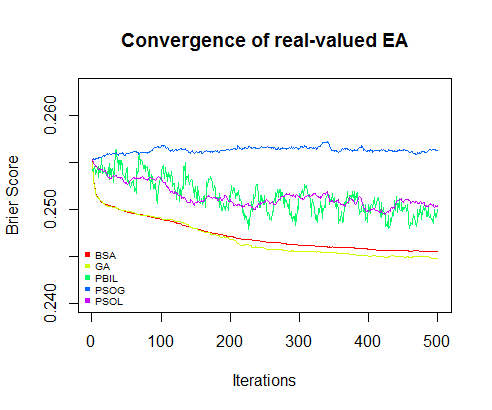
\includegraphics[width=\linewidth]{Conv_N_real_EA}
		%\caption{A subfigure}
		\label{fig:nr}
	\end{subfigure}
	\caption{Convergence Results of Experiments 1 and 2.}
	\label{fig:exp12}
\end{figure}

\begin{figure}
	\centering
	\begin{subfigure}{.5\textwidth}
		\centering
		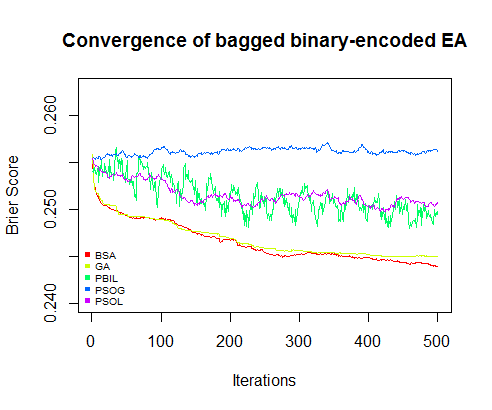
\includegraphics[width=\linewidth]{Conv_bin_bag}
		%\caption{A subfigure}
		\label{fig:bb}
	\end{subfigure}%
	\begin{subfigure}{.5\textwidth}
		\centering
		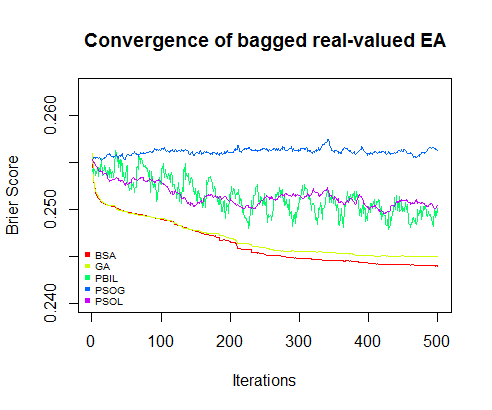
\includegraphics[width=\linewidth]{Conv_real_bag_EA}
		%\caption{A subfigure}
		\label{fig:br}
	\end{subfigure}
	\caption{Convergence Results of Experiments 1 and 2.}
	\label{fig:exp34}
\end{figure}

\begin{table}[ht]
	\centering
	\begin{tabular}{lccllcc}
		\hline
		Algorithms & ES (binary) & ES (real) & $\mid$ & Algorithms & ES (binary) & ES (real) \\ 
		\hline
		BSA1 & 5 & 26 && PSOG1 & 8 & 13 \\ 
		BSA2 & 3 & 13 & &PSOG2 & 6 & 14 \\ 
		BSA.BAG1 & 9 & 18 && PSOG3 & 5 & 7 \\ 
		BSA.BAG2 & 3 & 6 & &PSOG4 & 2 & 4 \\ 
		GA1 & 4 & 4 & &PSOG.BAG1 & 7 & 10 \\ 
		GA2 & 5 & 5 & &PSOG.BAG2 & 3 & 5 \\ 
		GA3 & 4 & 5 & &PSOG.BAG3 & 4 & 4 \\ 
		GA4 & 3 & 3 & &PSOG.BAG4 & 2 & 4 \\ 
		GA.BAG1 & 2 & 3 && PSOL1 & 4 & 5 \\ 
		GA.BAG2 & 3 & 4 && PSOL2 & 6 & 8 \\ 
		GA.BAG3 & 2 & 3 & &PSOL3 & 3 & 12 \\ 
		GA.BAG4 & 3 & 4 & &PSOL4 & 7 & 8 \\ 
		PBIL1 & 9 & 17 & &PSOL.BAG1 & 4 & 6 \\ 
		PBIL2 & 3 & 26 & &PSOL.BAG2 & 6 & 6 \\ 
		PBIL3 & 7 & 9 & &PSOL.BAG3& 2 & 7 \\ 
		PBIL4 & 7 & 9 && PSOL.BAG4 & 5 & 11 \\ 
		PBIL.BAG1 & 8 & 12 && SHC & 3 & \\ 
		PBIL.BAG2 & 5 & 16 && SHC.BAG & 11 & \\ 
		PBIL.BAG3 & 6 & 7 && HC & 2 & \\ 
		PBIL.BAG4 & 7 & 8 && HC.BAG & 6 & \\ 
		\hline
	\end{tabular}
	\caption{Ensemble Sizes Chosen by the EA}
	\label{tbl:es}
\end{table}

The algorithms yield strongly varying results in terms of ensemble sizes. Some variants pick as many as 26 of the 54 classifiers, whereas others decide on only 2 - 3. A complete overview can be found in Table \ref{tbl:es}. Some results by \cite{opitz1999popular} indicate that the marginal benefit of inclusion is highest for the first few models in the ensemble and decreases quickly \cite[p. 190]{opitz1999popular}. Even though the classifiers in the library can be considered diverse due to their wide parameter range, it is intuitive that after a certain number of RF and XGBoost models in the ensemble, the performance does not improve anymore and the errors increase. The correlation of performance and ensemble size which is evident from Figure \ref{fig:perfsize} is extremely interesting: For both the binary- and the real-coded versions, sparse solutions tend to yield better results. Still, the error rate increases quicker in the binary case. This should not come as a surprise because real-valued solutions may include many classifiers, many of them by a small weight only, so they do not decrease the performance. In the binary case, the weights are less likely to be arbitrarily small so any classifier in the ensemble has a larger relative weight. 

\begin{figure}[ht]
	\begin{center}
		\includegraphics[scale=0.8]{Perform_size}
		\caption{A scatterplot of the error rate on the ensemble size.}
		\label{fig:perfsize}
	\end{center}
\end{figure}

The complete results of the experiments can be found in Table \ref{tbl:perf}, where the columns refer to the performance on the validation and classification set. The best performing configurations for each of the two data sets are printed in boldface. When two scores were equal, both are emphasized. Overall, the real-valued solutions tend to perform slightly better than their binary counterparts. 
 
In training, the bagged GA yields the best results with BSA and the PSO-L being very comparatively in their error rate. Interestingly, the population size has opposing effects on the performance across algorithms. Overall, the GA performs better with a small population size whereas the increase of solution vectors in the population yields a performance increase for all others. As was somewhat expected after reading the paper by \cite{kennedymendes}, the PSO-G with a global information topology performs the worst out of all the configurations.

When compared to the baseline evaluations, the EAs do not measure up. All solutions, even the best solutions have a notable increase in the BS compared to the single best model. Even a simple average of the four best models outperforms 31 of the binary and 28 of the real-valued solutions. Interestingly, both HC and SHC suffer from bagging and yield best results on the full model library. HC maintains the error rate of the best performing model by only adding another classifier to the ensemble, with SHC also only considering three classifiers. Both the HC and SHC weigh the two classifiers more cleverly than the bagged GA1 and GA3 which also only include two classifiers.%PERCENTAG EWRONG

This paper also considered the problem of overfitting, so that the results of applying the ensemble weights to the classification data are surprising. Five binary and four real-valued solutions yield BS that are significantly lower than the single best classifier. HC and SHC only perform as good as the best model and do not lower the BS further.  

\begin{table}[ht]
	\centering
	\begin{tabular}{lcccc}
		\hline
		& \multicolumn{2}{c}{BS on Validation} & \multicolumn{2}{c}{BS on Classification} \\
		\cline{2-5}
		Algorithms & Binary & Real & Binary & Real \\ 
		\hline
		BSA1 & 0.2413 & 0.2466 & 0.2951 & 0.3007 \\ 
		BSA2 & 0.2396 & 0.2419 & \textbf{0.2945} & 0.2957 \\ 
		BSA.BAG1 & 0.2454 & 0.2446 & 0.2986 & 0.2980 \\ 
		BSA.BAG2 & 0.2396 & 0.2403 & \textbf{0.2945} & 0.2953 \\ 
		GA1 & 0.2416 & 0.2395 & 0.2954 & 0.2947 \\ 
		GA2 & 0.2413 & 0.2407 & 0.2951 & 0.2949 \\ 
		GA3 & 0.2406 & 0.2402 & 0.2948 & 0.2947 \\ 
		GA4 & 0.2430 & 0.2402 & 0.2966 & 0.2951 \\ 
		GA.BAG1 & \textbf{0.2393} & \textbf{0.2391} & 0.2946 & 0.2947 \\ 
		GA.BAG2 & 0.2445 & 0.2402 & 0.3008 & 0.2961 \\ 
		GA.BAG3 & \textbf{0.2393} & \textbf{0.2391} & 0.2946 & \textbf{0.2946} \\ 
		GA.BAG4 & 0.2445 & 0.2418 & 0.3008 & 0.2980 \\ 
		PBIL1 & 0.2516 & 0.2516 & 0.3051 & 0.3049 \\ 
		PBIL2 & 0.2396 & 0.2466 & \textbf{0.2945} & 0.3007 \\ 
		PBIL3 & 0.2469 & 0.2452 & 0.3017 & 0.3001 \\ 
		PBIL4 & 0.2467 & 0.2426 & 0.3000 & 0.2972 \\ 
		PBIL.BAG1 & 0.2513 & 0.2512 & 0.3054 & 0.3048 \\ 
		PBIL.BAG2 & 0.2458 & 0.2454 & 0.3003 & 0.2995 \\ 
		PBIL.BAG3 & 0.2485 & 0.2436 & 0.3029 & 0.2988 \\ 
		PBIL.BAG4 & 0.2467 & 0.2428 & 0.3000 & 0.2974 \\ 
		PSOG1 & 0.2489 & 0.2475 & 0.3051 & 0.3035 \\ 
		PSOG2 & 0.2482 & 0.2477 & 0.3047 & 0.3037 \\ 
		PSOG3 & 0.2460 & 0.2527 & 0.3022 & 0.3097 \\ 
		PSOG4 & 0.2619 & 0.2617 & 0.3195 & 0.3192 \\ 
		PSOG.BAG1 & 0.2506 & 0.2479 & 0.3071 & 0.3040 \\ 
		PSOG.BAG2 & 0.2486 & 0.2526 & 0.3028 & 0.3070 \\ 
		PSOG.BAG3 & 0.2479 & 0.2541 & 0.3047 & 0.3115 \\ 
		PSOG.BAG4 & 0.2619 & 0.2617 & 0.3195 & 0.3192 \\ 
		PSOL1 & 0.2452 & 0.2405 & 0.2978 & 0.2957 \\ 
		PSOL2 & 0.2464 & 0.2459 & 0.3002 & 0.3007 \\ 
		PSOL3 & 0.2409 & 0.2447 & 0.2951 & 0.2974 \\ 
		PSOL4 & 0.2481 & 0.2486 & 0.3038 & 0.3035 \\ 
		PSOL.BAG1 & 0.2479 & 0.2451 & 0.3047 & 0.3012 \\ 
		PSOL.BAG2 & 0.2482 & 0.2465 & 0.3012 & 0.3008 \\ 
		PSOL.BAG3 & \textbf{0.2393} & 0.2403 & 0.2946 & 0.2957 \\ 
		PSOL.BAG4 & 0.2470 & 0.2456 & 0.3028 & 0.2995 \\ \hline
		HC & 0.2389 & & 0.2948 & \\ 
		HC.BAG & 0.2401 &  & 0.2949 & \\
		SHC & 0.2390 & & 0.2948 & \\ 
		SHC.BAG & 0.2404 &  & 0.2949 & \\ \hline
		BEST & 0.2389 & & 0.2948 & \\
		AVRG & 0.2553 & & 0.3092 & \\
		BEST4 & 0.2406 & & 0.2947 & \\
		\hline
	\end{tabular}
\caption{Performance Results of Evolutionary Algorithms on Validation and Classification Data}
\label{tbl:perf} 
\end{table}




